\chapter{What Not to Do}
\label{chap:do_not}

This chapter is devoted to listing a bunch of \emph{horrible}
things to do;
we list them here precisely because you should \emph{never}
do any of these things.

\section{General Advice}

\begin{itemize}
\item \textbf{Do not ``roll your own crypto.''}
    It is always a good idea to use software that professional cryptographers
        have written.
    It is a bad idea to write your own \gls{encryption scheme},
        \gls{signature} scheme,
        \gls{hash function}, \dots
    Use something written by experts.
    That library should have been written by someone with many years
        of experience in cryptography and it should have been vetted
        by other people as well.

    Along those lines is a quote from Bruce Schneier
    in 1998~\cite{SchneierBlog1998}:

\begin{quote}
    Anyone, from the most clueless amateur to the best cryptographer,
    can create an algorithm that he himself can't break.
    It's not even hard. What is hard is creating an algorithm
    that no one else can break, even after years of analysis.
\end{quote}

    Bad things can happen when you do not know what you are doing;
    see Figure~\ref{fig:xkcd_security_holes} and~\cite{SchneierBlog2008}.

\begin{figure}[t]
\centering
    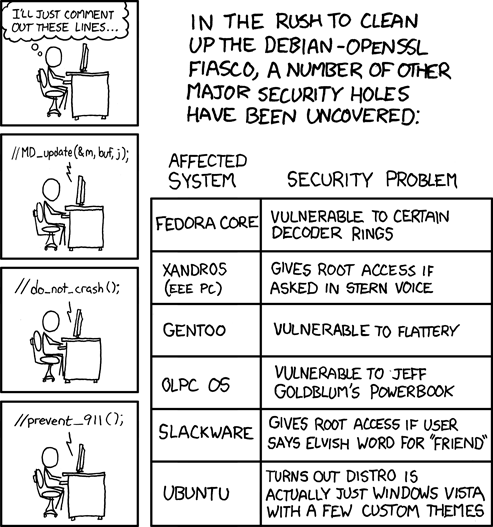
\includegraphics[width=0.75\textwidth]{figures/xkcd/xkcd_424_security_holes.png}
    \caption[\texttt{xkcd} Security Holes]{Here is an example
        of the fragility of cryptography in the real world.
        Created by Randall Munroe on \texttt{xkcd};
        posted online at \url{https://xkcd.com/424/}.
        }
    \label{fig:xkcd_security_holes}
\end{figure}


\item \textbf{Do not randomly combine cryptographic primitives
    to arrive at something you think solves the problem.}
    Take the time to think about \emph{exactly} what you are trying to do.
    If you are wanting to store passwords,
    then use a using a \gls{kdf} designed
    for password storage
    and not a standard \glsfirst{hash function};
    both are useful but serve different purposes.

\item \textbf{Whenever possible, do not use randomized algorithms.}
    There are many problems which may arise when using
        random number generators.
    Thus, whenever possible, use deterministic algorithms.
    There may be times when algorithms requiring randomness
    can be reworked to use ``deterministic randomness'' based on
    \glsfirstplural{hash function}.
    This would be the preferred method;
    see~\cite{rfc6979} for a reference to ``deterministic randomness''
    in \glspl{signature}.

\item \textbf{Do not use classical algorithms.}
    If any real security is required, do not \emph{ever} use
    classical algorithms like substitution or transposition ciphers.
    All classical ciphers can easily be brute-forced and may
    be broken given enough ciphertext.
    A couple references for attacking classical ciphers using
    frequency analysis are
    \cite[Chapter 1.3]{IntroModernCrypto}
    and \cite[Chapter 1.1]{IntroMathCrypto}.

\item \textbf{The only \gls{encryption scheme} with \gls{perfect security}
    is the \gls{otp}.}
    Any perfectly secure encryption scheme is equivalent to the
    \gls{otp}~\cite[Theorems 2.10 and 2.11]{IntroModernCrypto}.
    Anyone who claims to have a perfectly secure algorithm
    that is better than the \gls{otp} is \emph{lying}.

\item \textbf{Do not use ``security through obscurity'' or
    assume a secret algorithm will be sufficient for security.}
    This goes against
    \emph{Kerchoff's principle}~\cite[Page 5]{IntroModernCrypto}:

\begin{quote}
    The cipher method must not be required to be secret,
    and it must be able to fall into the hands of the enemy
    without inconvenience.
\end{quote}

\end{itemize}

\section{Symmetric Key Encryption}

\begin{itemize}
\item \textbf{Do not use ECB-mode when encrypting with a \gls{block cipher}.}
    ECB stands for \emph{Electronic Codebook}.
    This method should \emph{never} be used when performing
    encryption with a \gls{block cipher}.
    It leaks too much information; see Chapter~\ref{ssec:block_cipher}
    for more information.
\item \textbf{Do not use DES.}
    DES stands for \emph{Data Encryption Standard} and is a \gls{block cipher}.
    The small key size allows it to be easily broken~\cite{rfc4772}.
    The \emph{only} reason to ever use it is because its use is required
    for compatibility with legacy systems.
\item \textbf{Do not use RC4.}
    RC4 is a cryptographically-broken \gls{stream cipher}~\cite{rfc7465};
    see Chapter~\ref{ssec:stream_cipher} for more information.
\item \textbf{Do not use Blowfish.}
    Blowfish is an old \gls{block cipher},
    and in 2007 its author recommended~\cite{SchneierNews2007}
    switching from Blowfish~\cite{BlowfishAlg} to Twofish~\cite{TwofishAlg}.
\end{itemize}

\section{Cryptographic Hash Functions}

\begin{itemize}
\item \textbf{Do not use \MDFive{}.}
    \MDFive{} is a cryptographically-broken \gls{hash function}~\cite{rfc6151}.
    The \emph{only} reason to ever use it is because its use is required
        for compatibility with legacy systems.
\item \textbf{Do not use \ShaOne{}.}
    See the reasons above about why \MDFive{}
    should not be used~\cite{rfc6194,cryptoeprint:2020/014}.
\item \textbf{Do not use PBKDF2 as a \gls{kdf}.}
    It has been shown to provide insufficient protection
    when protecting passwords~\cite{blocki2018economics}.
\item \textbf{Do not use \texttt{bcrypt} as a \gls{kdf}.}
    It has also been shown to provide insufficient protection
    when protecting passwords~\cite{blocki2018economics}.
\end{itemize}

\section{Cryptographically-Secure Pseudorandom Number Generators}

\begin{itemize}
\item \textbf{Do not use Dual\_EC\_DRBG.}
    The standard algorithm~\cite[Section~10.3.1]{NIST-SP-800-90A}
    is believed to have a backdoor~\cite{BernsteinDualEC}
    and was removed in a later version~\cite{NIST-SP-800-90ARev1}.
\item \textbf{Do not use non-cryptographic PRNGs for cryptographic protocols.}
    Cryptographic protocols \emph{require} cryptographically-strong
    pseudorandom numbers;
    these numbers come from a \gls{csprng}.
    The numbers provided by non-cryptographic PRNGs
    \emph{are not sufficiently random}~\cite{marsaglia1968random,bouillaguet2020practical}.

    Here is a non-exhaustive list of non-cryptographic PRNGs:
    Linear Congruential Generator (LCG), Permuted Congruential Generator (PCG),
    Mersenne Twister.
    \emph{None} of these PRNGs should \emph{ever be used}
    in cryptographic situations.
\end{itemize}

\section{Public Key Encryption}

\begin{itemize}
\item \textbf{Do not use publish the private key.}
    This should go without saying.
\end{itemize}

\section{Digital Signatures}

\begin{itemize}
\item \textbf{Do not use publish the signing key.}
    This should go without saying.
\end{itemize}

